\documentclass[10pt,twocolumn,letterpaper]{article}

% 私自身のもの
\usepackage{booktabs}
% \usepackage{caption}
% \captionsetup[table]{skip=8pt}   % テーブルのみに影響
\usepackage{stfloats}  % これをプリアンブルに追加
\usepackage{float}
\usepackage{xeCJK}  % Supports Simplified & Traditional Chinese
\setCJKmainfont{IPAMincho} 

\usepackage{cvpr}
\usepackage{times}
\usepackage{epsfig}
\usepackage{graphicx}
\usepackage{amsmath}
\usepackage{amssymb}

% 他のパッケージはここでhyperrefの前に含めてください。

% hyperrefをコメントアウトしてからまたアンコメントした場合は、
% latexを再実行する前にegpaper.auxを削除してください。(またはlatexの最初の実行時に'q'を押してください)
% run, let it finish, and you should be clear).
\usepackage[breaklinks=true,bookmarks=false]{hyperref}

\cvprfinalcopy % *** Uncomment this line for the final submission

\def\cvprPaperID{****} % *** Enter the CVPR Paper ID here
\def\httilde{\mbox{\tt\raisebox{-.5ex}{\symbol{126}}}}

% Pages are numbered in submission mode, and unnumbered in camera-ready
%\ifcvprfinal\pagestyle{empty}\fi
\setcounter{page}{1}
\begin{document}

%%%%%%%%% TITLE
\title{ECDOデータ駆動型入門パート1/2:発熱性核-マントル分離ジャニベコフ振動(ECDO)「地球反転」理論の現在の理解}

\author{ジュノ\\
2025年2月発行\\
ウェブサイト(論文はここからダウンロード):\href{https://sovrynn.github.io}{sovrynn.github.io}\\
ECDO研究リポジトリ:\href{https://github.com/sovrynn/ecdo}{github.com/sovrynn/ecdo}\\
{\tt\small junhobtc@proton.me}
% すべての著者が同じ機関に所属している論文の場合は、
% 以下の行を閉じかっこ ``}'' まで省略してください。
% 追加の著者やアドレスは ``\and'' で追加できます。
% 2人目の著者のように書くことができます。
% スペースを節約するために、メールアドレスまたはホームページのいずれか一方のみを使用してください。
% \and
% Craig Stone\\
% Institution2\\
% Institution2の住所の1行目\\
% {\tt\small secondauthor@i2.org}
}

\maketitle
%\thispagestyle{empty}

%%%%%%%%% ABSTRACT
\begin{abstract}
2024年5月、 倫理的懐疑論者「The Ethical Skeptic」と名乗る匿名のオンライン著者が、Exothermic Core-Mantle Decoupling Dzhanibekov Oscillation(ECDO)と呼ばれる画期的な理論 \cite{0}\cite{1} を発表しました。この理論は、地球が過去に自転軸の急激かつ壊滅的な変動を経験し、その結果、回転慣性によって大洋が大陸にあふれ、世界的な大洪水が引き起こされた可能性を示唆しています。さらに、同様の地軸反転が再び差し迫っていることを示す地球物理学的な過程とデータも提示されています。このような壊滅的な洪水や終末的な予測自体は新しいものではありませんが、ECDO理論は、科学的かつ現代的で学際的、かつデータに基づくアプローチにより、他とは一線を画す説得力を持っています。

本論文は、6ヶ月間の独立した研究 \cite{2,20} に基づくECDO理論に関する2部構成の要約の第1部です。本論文では、3つの主要なポイントを強調しています。

\begin{flushleft}
\begin{enumerate}
    \item ECDOのような「地球反転」は、洪水神話や大規模な大陸の洪水を示す地質学的証拠により、人類の近年の歴史の中で複数回発生している。
    \item 過去の地球反転のおおよその方向と規模を特定することができる。
    \item 最近の地磁気および地球物理学的データは、別の地球反転が差し迫っている可能性を示唆しており、気候変動は人間ではなく地球内部の変化によって引き起こされている可能性がある。
\end{enumerate}
\end{flushleft}

さらに、本論文ではECDO理論で提唱された「地球反転」を引き起こす物理現象についても取り上げる。

本論文では、客観性を保つために厳密なデータに注目し、説得力はあるが推測的な理論部分を避け、人類が急いで調査すべき重要なテーマであることを強調する。
\end{abstract}

%%%%%%%%% BODY TEXT
\section{序章}

大洪水の歴史は新しいものではなく、事実上、文明のすべての揺りかごを網羅し、世界中の主要な文化で見られる。267件の洪水伝説をまとめてプロットすると(図 \ref{fig:1}、\cite{3})、人類が居住する地球のほぼすべての地域に洪水の物語が存在することがわかる。

% \begin{figure}[h]
% \begin{figure}[b]
\begin{figure}[h]
\begin{center}
% \fbox{\rule{0pt}{2in} \rule{0.9\linewidth}{0pt}}
   \includegraphics[width=1\linewidth]{b.png}
\end{center}
   \caption{世界中の洪水伝承の分布 \cite{3}.}
\label{fig:1}
\label{fig:onecol}
\end{figure}

これらの洪水伝承を詳しく見ると、これらは単なる通常の洪水ではなく、大陸を一掃した洪水を伴う破壊的な大災害であったことがわかる。

\subsection{ネイティブアメリカンの大災害伝承}

ネイティブアメリカンの伝承には、地球の大災害について最も生々しい記録が含まれている。アリゾナ州北東部に住むネイティブアメリカン部族のホピ族は、\textit{"...ソトクナンはアリの民に選ばれた人々のために地下世界を開けるよう命じました。人々が無事に地下に入ると、ソトクナンは双子のポカンホヤとパロンガウホヤに、地球を正しく回転させるために世界の軸の北端と南端に配置されていた持ち場を離れるよう命じました。\textbf{双子が持ち場を離れてしまうと、誰も制御する者がいなくなった世界はバランスを崩し、めちゃくちゃに回転した後、二度転がりました。} 山々は大きな音と共に海へ落ち、海や湖は陸地にあふれました。そして、冷たく生命のない空間を世界が回転するうちに、全てが凍って固い氷となりました"} \cite{4}.

これらの伝承の多くは、洪水の規模がいかに大きかったかを正確に描写しており、海が上昇して最も高い山の頂上を除いて全てを水没させたことを伝えている。ワシントン州に住むスココミッシュ・インディアンは、\textit{"偉大な精霊は人間と動物の邪悪さに怒り、善良な動物と一人の善良な男とその家族を残して、地上のすべてを滅ぼすことに決めました。偉大な精霊の指示で、その男は雲に矢を放ち、さらにその矢にまた矢を放っていき、雲から地面まで矢のロープを作りました。善良な動物や人々が登りました。悪い動物やヘビも登ろうとしましたが、男はロープを壊しました。\textbf{その後、偉大な精霊は何日も雨を降らせ、タコマ山(レーニア山)の雪線まで水浸しにしました。} 悪い人々や動物が全て溺れた後、偉大な精霊は雨を止め、水がゆっくり引いて善良な人や動物は降りてきました"} \cite{3}. 参考までに、レーニア山は標高4392.5メートルのワシントン州にある活火山である。

ワシントン州のマカ族インディアンの洪水伝説は、「非常に暖かい」水による多段階の洪水を具体的に言及しており、これが通常の洪水ではなかったことを示しています: \textit{「海は岬を切り離すほどに高くなった。それから四日後には引いて、ネアベイは完全に干上がった。その後、再び海が上昇し、山頂以外すべてを覆った。\textbf{水は非常に温かかった。}カヌーに荷物を積み込んだ人々は、はるか北へ流された。カヌーが木に引っかかって多くの人が亡くなった。さらに四日後、海は元に戻り、人々はずっと北の地にいることに気づいた。そこに彼らの子孫はいまも住んでいる。」} \cite{3}。

\subsection{中国の大変動の伝承}

太平洋の反対側では、現代中国文明は大洪水によって始まったとされている。紀元前2000年頃と推定される夏王朝は、禹が鯀禹の大洪水を治めて建てた王朝である \cite{6}。その時代について、\textit{「……奇跡的な出来事として、十日間太陽が沈まず、森は燃え上がり、無数の忌まわしい虫が発生した……天にまで届くほどの巨大な波が中国の大地に押し寄せた。\textbf{『水は高い山まで達し、丘は全く見えなかった』}……『氾濫する水は破壊的である』と皇帝は言った。『その広がりは山々を包み込み、高所をも覆い、天を脅かすほどの洪水だ』皇帝は、山と山の谷間にたまった水を流すため、あらゆる努力をするよう命じた。幾年もの間、民は野や谷を水で満たさないように溝を掘り、排水に努めたが、長い間全ての努力は無駄だった。この重大な事業の責任者、鯀は失敗の責任で死刑になり……彼の息子・禹だけが土地の排水に成功した。この偉業が高く評価され、禹は舜の次に皇帝となった」} \cite{5}。

洪水は中国全土を覆っただけでなく、方位や太陽や月の動きを再測定する必要があったようで、これは洪水の際に地球の自転が変化した可能性も示唆する:\textit{ \textbf{「この皇帝は学者たちを中国各地やインドシナにも送り、太陽の昇る沈む方向や星の動きを観察させて、北・西・東・南の方角を確かめさせた。}また、天文学者には季節の長さを調べ、新しい暦を作るよう命じた……『これにより堯(ヤオ)は、天の規範に従い、太陽、月、星、黄道の運行を計算し、四季を民に分かりやすく伝えよと命じた』」} \cite{5}。

中国史における大変動の記録は、実は夏王朝よりもはるか以前、三皇五帝の時代にまで遡る \cite{7}。三皇のひとりであり中国神話の創造神でもある女媧は、大洪水と地球の自転変化の際に世界を救った:\textit{「力強い神同士の争いがあり、戦いの末、水神の共工は敗色濃厚となって不周山に頭をぶつけた。不周山は天を支える柱であり、\textbf{柱が崩れて天は西北に傾き、地は東南に沈んだ。}そのため、大火災、洪水、獰猛な人食い獣の出現など様々な災厄が起きた。女媧は大亀の足を切り取って柱の代わりにし、七色の石で破れた天を塞いだが、完全には元には戻せなかった」} \cite{8}。

\subsection{ヨーロッパ、マヤ、中東、東南アジアの大変動伝承}

本稿ではとてもすべての大変動伝説を紹介しきれないため、著名なものをいくつか挙げるにとどめる。ギリシャ文学にはデウカリオーン、オギュゲス、ダルダノスの三つの洪水伝説がある \cite{9,10}。デウカリオーンの洪水では、\textit{「九日間の洪水の後、世界は滅び、方舟は標高2,457メートルのパルナッソス山頂にとどまった」}と言われる \cite{11}。マヤ神話では、現行の太陽の前に四つの太陽があり、第四の太陽「カルチウトリクエ」の時代は紀元前3100年頃の大洪水とともに終わり、現在の第五の太陽が生まれたとされる \cite{12}。中東では、聖書のノアの洪水やバビロニアの『ギルガメシュ叙事詩』にも類似の大洪水譚がある \cite{13}。東南アジアにも洪水伝説は多く、たとえばインドネシアのオッ・ダヌム族には、\textit{「昔、大洪水が多くの人を溺死させた。少数の人々だけが最も高い山へ船で逃れ、生き残った。三ヶ月後に水が引いた」}という伝承が残る \cite{3}。彼らが住むボルネオ島の最高峰は標高4,095メートルである。

\begin{figure*}[b]
\begin{center}
% \fbox{\rule{0pt}{2in} \rule{.9\linewidth}{0pt}}
\includegraphics[width=1\textwidth]{marine.jpg}
\end{center}
   \caption{海洋性化石、海水、塩湖/塩鉱の世界地図 \cite{15,16,86,87}.}

   \label{fig:2}
\end{figure*}

\subsection{統計的な大災害物語の分析}

明らかに、これらの物語は、他の種類の壊滅的な地球物理的な力を伴うことが多い大洪水を描写しています。117件の大災害物語の分析(表\ref{tab: 1})によれば、火災嵐、地形の変化、地球の自転の変化などが大洪水とともに発生したと記録されていることが多いです\cite{14}:

\begin{table}[ht]
\begin{center}
\renewcommand{\arraystretch}{1.2}  % Optional, to increase row spacing
\begin{tabular}{|l|c|c|}
\hline
\textbf{大災害の種類} & \textbf{件数} & \textbf{発生率\%} \\
\hline\hline
大洪水・洪水            & 84 & 71.79 \\
火災・火災嵐            & 39 & 33.33 \\
地形の変化              & 29 & 24.79 \\
星の混乱                & 15 & 12.82 \\
天空の崩壊              & 15 & 12.82 \\
長期間の暗闇            & 14 & 11.97 \\

失われた土地や湖 & 12 & 10.26 \\
サイクロン性の風 & 10 & 8.55  \\
地軸/回転の変化 & 9 & 7.69  \\
川/湖/海の沸騰 & 8 & 6.84 \\
\hline
\end{tabular}
\end{center}
\caption{物語における壊滅的な影響の発生件数}
\label{tab: 1}
\end{table}

% \begin{table}[h]
%     \centering
%     \renewcommand{\arraystretch}{1.2}
%     \begin{tabular}{l c c}
%         \toprule
%         \textbf{カタクリズムの種類} & \textbf{件数} & \textbf{発生率(\%)} \\
%         \midrule
%         大洪水 & 84 & 71.79 \\
%         大火災 & 39 & 33.33 \\

%         地形の変化 & 29 & 24.79 \\
%         % 雷/騒音/轟音 & 16 & 13.68 \\
%         恒星の混乱 & 15 & 12.82 \\
%         崩壊した空 & 15 & 12.82 \\
%         長引く闇 & 14 & 11.97 \\
%         失われた土地と湖 & 12 & 10.26 \\
%         % 空からの落下:雹、金、砂利、石、塵 & 11 & 9.40 \\
%         サイクロン状の風 & 10 & 8.55 \\
%         % 稲妻 & 10 & 8.55 \\
%         % 天体来訪者の描写 & 9 & 7.69 \\
%         % 天体来訪者の分裂と落下 & 9 & 7.69 \\
%         地軸/回転の変化 & 9 & 7.69 \\
%         沸騰する川/湖/海 & 8 & 6.84 \\
%         % 空からの落下:可燃性/樹脂状物質 & 7 & 5.98 \\
%         % 洪水以前の文明への言及 & 7 & 5.98 \\
%         % 空からの落下:鉄分物質 & 6 & 5.13 \\
%         % 毒された大気 & 4 & 3.42 \\
%         % 氷の到来 & 3 & 2.56 \\
%         % 植生への影響 & 3 & 2.56 \\
%         % 蒸気 & 2 & 1.71 \\

%         \bottomrule
%     \end{tabular}
%     \caption{物語における壊滅的影響の発生}
%     \label{fig: 2}
% \end{table}

世界中の多くの独立した文化から生じた洪水物語の特殊性と、他の壊滅的出来事に関する一致する物語は、これらの洪水物語が実際に起きた災害の直接的な記録である可能性を示唆している。

\section{海洋性洪水に関する物理的証拠}

洪水物語を裏付けるものとして、地球の大陸表面に広がる広範な海洋浸水の物理的証拠がいくつか存在する。最も直接的な証拠としては、塩分(塩水、塩田、塩鉱山)や海洋(海洋性)化石があり、これらは地球の大陸の広い範囲を覆っている。図\ref{fig:2}は、塩水(青)、塩田と塩鉱山(茶色)、および海洋化石\cite{15,16,86,87}の分布を示し、これらの海洋浸水の指標の広がりを示している。

% \begin{figure}[t]
% \begin{center}
% \fbox{\rule{0pt}{2in} \rule{1\linewidth}{0pt}}
%    % \includegraphics[width=1\linewidth]{b.png}
% \end{center}
%    \caption{TODO ここには塩と海洋化石の2次元グラフィックが表示される}
% \label{fig:1}
% \label{fig:onecol}

% \end{figure}

塩水を含む最も興味深い地域のいくつかは、チベットのヒマラヤ高地と南米アンデス山脈であり、どちらの地域も平均標高は4000メートルである。前者は図\ref{fig:3}に示されている。チベットの洪水伝説によれば、\textit{「\textbf{チベットはほとんどが水没した}が、神ギャ(Gya)が生存者に憐れみをかけて、ベンガルを通して水を引き、教師たちを送って人々を文明化した。それまで人々は猿同然だった。」}\cite{3}とされている。ペルーの神話では、山の造成が山を覆う大洪水とともに起こったと描写されている:\textit{「羊飼いと6人の子供たちは、できる限りの食糧と羊を集め、非常に高い山アンカスマルカの頂上に持って行った。 \textbf{洪水の水が上昇するにつれて、山も高くなり、頂上は決して水没せず、その後、山は水とともに沈んだ。} 6人の子供たちは洪水の後にこの地方に人々を再び増やした。」}\cite{3}。

\begin{figure}[t]
\begin{center}
% \fbox{\rule{0pt}{2in} \rule{0.9\linewidth}{0pt}}
   \includegraphics[width=1\linewidth]{tibet.jpg}
\end{center}
   \caption{ヒマラヤの地形図。塩水(ティール)、乾燥塩(白)、および海洋化石(赤)を示す\cite{15,16,86,87}。}
\label{fig:3}
\label{fig:onecol}
\end{figure}

斉一説的な地質学派は、塩や海洋化石のような異常現象を、数百万年に及ぶ長期間のプロセスの結果と考えているが、人類の洪水伝説はその考え方に疑問を投げかけるものだ。もし本当に海が大陸を覆う洪水を起こしたのであれば、高地の広大な地域に塩水や海洋化石が容易に見つかるのは、まさに予想されることである。

% \begin{figure*}[b]
% % \begin{figure*}[t]
% \centering
% \includegraphics[width=0.8\textwidth]{khafre.jpg}

% \caption{持続的かつ一時的な海洋の移動によって引き起こされる差別的でパターン化されたカルスト侵食の図。}
% \label{fig:1}
% \end{figure*}

\begin{figure*}[t]
\begin{center}
\includegraphics[width=0.85\textwidth]{khafre.jpg}
\end{center}
   \caption{持続的かつ一時的な海面上昇によって引き起こされる差別的でパターン化されたカルスト侵食を示す図 \cite{27}。}
\label{fig:4}
\end{figure*}

\subsection{その他の物理的異常}

斉一論的科学では説明できない多数の異常が存在する。泥の中に埋もれて完璧に保存され、何千年も経った後でも肉がまだ食べられる冷凍マンモス \cite{17,18,19}、北アメリカに広がる2.4百万km$^2$に及ぶ大規模な水平堆積した堆積物のシート \cite{21}、メガカレントリップル地形 \cite{22}、および数百キロメートル離れた場所から来た迷子石が山頂に載っている現象 \cite{23,26} などは、現代の斉一論的地質学が「長期間にわたる自然なプロセス」という包括的な説明で単純に片付けてしまう現象の一部に過ぎない。これらの異常は、災害的な地球物理学的力によって最もよく説明でき、本論文の第2部で詳しく探求する。

さらに、古地磁気データに基づき、地磁気極の偏位や逆転が地球の周期的な現象として広く認められている \cite{35,40,41}。しかし、現代科学ではこれらの極逆転がなぜどのように起こるのか正確には説明できていない。

\section{ECDOとギザのピラミッド}

ギザのカフラー王とクフ王のピラミッドは、倫理的懐疑論者(The Ethical Skeptic)のECDO論文\cite{27}における重要な焦点の一つである。これらのピラミッドは、一時的かつ持続的な海洋浸水の証拠を提供するだけでなく、地球のECDO反転の可能性のある方向を示しており、我々の祖先が地球規模のカタストロフィを測定し、その知識を巨大かつ高度に設計された石造構造物に組み込む技術を持っていたことを示唆している。これら二つのピラミッドは、紀元前2500年頃、ファラオのクフとカフラーの墓として建てられたとされ、どちらも北エジプトのほぼ(30 N, 31 E)に位置している。基底部は200メートルを超え、高さは約140メートルである。クフ王のピラミッドは、約230万個の石灰岩ブロック(平均して2トン以上の重さ)を使用して建設された\cite{24, 25}。

これらのピラミッドの起源には多くの不確実性が存在し、倫理的懐疑論者(The Ethical Skeptic)はその論文でこの点について述べている。彼は、従来のピラミッドに関する物語には多くの矛盾点があることを指摘し、少なくともその年代や歴史に関して大きな混乱があることを示唆している:

\begin{flushleft}
\begin{itemize}
    \item 近くで発見された古代のモルタルや墓泥棒の道具の放射性炭素年代測定によれば、これらのピラミッドは従来考えられているよりもはるかに古く建設された可能性が高い。
    \item クフ王のピラミッド内部のいわゆる採石場の印は、その位置、材料、保存状態、エジプト象形文字の使用、発見の時期や経緯において不審な点があり、偽造の可能性を示唆している。それらは、ピラミッド内の別の場所で発見された他の本物の古代のオーカーの印とは異なっている。
    \item 近くのスフィンクスに見られる異なるカルスト侵食の様子は、その建設に関する従来の物語と一致しない。
\end{itemize}
\end{flushleft}

\begin{figure*}[b]
\begin{center}
\includegraphics[width=0.85\textwidth]{shafts.jpg}
\end{center}
   \caption{倫理的懐疑論者(The Ethical Skeptic)が、ECDO現象のための三分割地球物理観測所であったと提案するクフ王のピラミッド内部の通路と部屋\cite{28}。}
\label{fig:5}
\end{figure*}
倫理的懐疑論者(The Ethical Skeptic)の論文における主要な研究対象の一つは、図4に示されるカフラーピラミッドの外壁にみられる差動的なパターン化された侵食です。 \ref{fig:4} ピラミッドの先端部は、かつてピラミッド全体を覆っていた元の柔らかいトゥラ石灰岩の外装層を維持しています。この石灰岩の外装層の先端部は軽く風化していますが、その直下には狭く激しくカルスト侵食を受けた層があり、ピラミッドの内部構造ブロックに使用された硬いモース7のモッカタム石灰岩が露出しています。その下には、ピラミッドの本体がモース硬度4のトゥラ石灰岩層を保持しています。重要な点は、ピラミッドの外装に使用された軟らかいトゥラ石灰岩(CaCO3)が、適切な条件下で水に溶解する点です。倫理的懐疑論者(The Ethical Skeptic)は、硬いモッカタム石灰岩で止まる選択的な重度のカルスト侵食層、先端の角の波状侵食、およびピラミッドの先端のわずかな風化と下部の重度のカルスト侵食の差を、海洋水位の上昇が持続的に起こり、その後急速に後退した明確な証拠として挙げています \cite{27}。

% \begin{figure}[t]
% \begin{center}
% % \fbox{\rule{0pt}{2in} \rule{0.9\linewidth}{0pt}}
%    \includegraphics[width=1\linewidth]{khafre.jpg}
% \end{center}
%    \caption{A diagram of the differential karst erosion caused by a sustained, temporary oceanic displacement.}
% \label{fig:1}
% \label{fig:onecol}
% \end{figure}

\begin{figure*}[t]
\begin{center}
% \fbox{\rule{0pt}{2in} \rule{.9\linewidth}{0pt}}
\includegraphics[width=1\textwidth]{drawing.jpg}
\end{center}
   \caption{提案されたECDO回転が東経31度子午線に沿って北へ104度進む様子を示した図。十字は東側と西側のピボット位置、赤いマーカーはクフ王のピラミッドを示している。}
\label{fig:6}
\end{figure*}

倫理的懐疑論者(The Ethical Skeptic)はまた、調査の中でクフ王ピラミッドの内部構造と状態(図\ref{fig:5})にも強く注目している\cite{28}。クフ王ピラミッドには複数の部屋(王の間、王妃の間、地下室)、さまざまな通路とシャフト、さらにいわゆる「通気シャフト」と呼ばれる2対のシャフトがあり、それぞれ王の間と王妃の間から1対ずつ伸びている\cite{29,30}。本論文では、倫理的懐疑論者(The Ethical Skeptic)の調査の中でも最も重要な部分――すなわち2対の「通気シャフト」の方向と設計についてのみ扱う。これらは、地球のECDO反転の方向に関する重要な情報をコード化しているためである。

% \begin{figure}[b]
% \begin{center}
% % \fbox{\rule{0pt}{2in} \rule{0.9\linewidth}{0pt}}
%    \includegraphics[width=1\linewidth]{shafts.jpg}
% \end{center}
%    \caption{クフ王ピラミッドの内部シャフトと部屋。倫理的懐疑論者(The Ethical Skeptic)は、これが三分割された地球物理学的観測所であったと考えている。}
% \label{fig:1}
% \label{fig:onecol}
% \end{figure}

ここでの鍵は、これらのシャフトが非常に正確に特定の方向を指すように設計されていることを理解することである。まず、両方のシャフトは現在、直接的に北と南を指している。さらに、それぞれ内角104度で建設されている。

しかし最も示唆的な手がかりは、王妃のシャフトの1つの内部に刻まれている天体星図である。この星図は、春分点歳差運動に基づいて、およそ紀元前9600年から9200年の天体北極の方向を中心に描かれている\cite{28}。これはシャフトの向きが意図的であり、建造時点で王と王妃の間から伸びる一対のシャフトが天体北極を指していたことを示唆している。ここで疑問が生じる――ではもう一方のシャフトの先端はどこを指し、なぜ両方とも104度という角度で作られていたのか?倫理的懐疑論者(The Ethical Skeptic)は、これらが104度のECDO反転後の天体北極に合わせるために建設されたのだと提案している。

% \begin{figure}[t]
% \begin{center}
% % \fbox{\rule{0pt}{2in} \rule{0.9\linewidth}{0pt}}

%    \includegraphics[width=1\linewidth]{star-stone.jpg}
% \end{center}
%    \caption{女王の星のシャフトの1つに刻まれた岩に描かれた天体の星図の図 \cite{28}.}
% \label{fig:1}
% \label{fig:onecol}
% \end{figure}

\section{第31子午線に沿った104度の回転の証拠}

\begin{figure}[t]
\begin{center}
% \fbox{\rule{0pt}{2in} \rule{0.9\linewidth}{0pt}}
   \includegraphics[width=0.95\linewidth]{laj.jpg}
\end{center}
   \caption{(a) アイスランド海盆偏移 および (b) ラシャンプ偏移の仮想地磁気極軌道 \cite{35}.}
\label{fig:7}
\label{fig:onecol}
\end{figure}

\begin{figure*}[t]
\begin{center}
% \fbox{\rule{0pt}{2in} \rule{.9\linewidth}{0pt}}
\includegraphics[width=0.95\textwidth]{biodiversity.jpg}
\end{center}
   \caption{世界の主要な砂漠と交互に現れる生物多様性ホットスポットの図 \cite{28}。}
\label{fig:9}
\end{figure*}

\begin{figure}[t]
\begin{center}
% \fbox{\rule{0pt}{2in} \rule{0.9\linewidth}{0pt}}
   \includegraphics[width=1\linewidth]{meinesz3.jpg}
\end{center}
   \caption{地殻における剪断パターンの図示 \cite{36}.}
\label{fig:8}

\label{fig:onecol}
\end{figure}

倫理的懐疑論者(The Ethical Skeptic)は、地球がクフ王のピラミッドとその二重のシャフトがある第31子午線に沿って、繰り返し104度の反転を経験すると提案している。図\ref{fig:6}は、予測された回転、および東(インドネシア、東経121度)と西(南米、西経59度)の「ピボット」、すなわち第31子午線に沿った反転の後に位置が変わらない2地点を示している。地球がこの新しい状態へと回転した後、数十年から数世紀の間はそのまま留まり、やがて現在の「通常」状態へ戻ると予測されている \cite{150}。

特に関連性の高い大災害の物語として、紀元前5世紀に生きた古代ギリシャでもっとも有名な歴史家ヘロドトスによるものがある \cite{31}。彼の著書『エジプト誌』では、エジプトの祭司が彼に語った内容を次のように記している:\textit{「…最初の王からヘファイストス神の祭司で最後に治めたこの王まで、人間の世代は三百四十一世代あった…しかし三百世代の人間は一万年に等しく、一世代三十三年と見なされる…それゆえ一万一千三百四十年間において、人間の姿をした神は現れなかったと言った。それ以前にも以後にもエジプトに王が現れた際、そういうことは何もなかったと報告している。\textbf{この間に、太陽は四度その慣れ親しんだ昇る場所を変え、今沈んでいるところから二度昇り、今昇っているところから二度沈んだ};そしてその間、エジプトでは地から生じるものも、川からもたらされるものも、病気や死に関することも、何も変わらなかった」} \cite{32}。ヘファイストスの祭司は、新アッシリア帝国の王センナケリブと同時代人であり、紀元前7世紀初頭に位置づけられるとヘロドトス自身が述べている \cite{32,33,34}。

この話が重要なのは、太陽がエジプトで動いたとき、\textit{特に昇る場所と沈む場所を入れ替えた}ことを示しているからである。これは、エジプトが180度反転し、類似した緯度にとどまった場合にのみ起こり得る。ピラミッドの設計や次節で扱うデータを考慮すると、エジプトが地球の新たな位置に回転する子午線、すなわち第31東経子午線上にある可能性が推測できる。

エジプトは、太陽が明確に昇降場所を入れ替えたという話が伝わる\textit{唯一の}地域である。実際、地球の回転方向を明確に述べているもう一つの話は中国の女媧(Nüwa)の物語だけであり、そこでは\textit{「柱が倒れて天が北西に傾き、地が南東にずれた」}とされている \cite{8}。この回転方向も提案された方向と一致している。

\subsection{第31子午線に沿う104度回転の物理的証拠}

この回転方向を裏付ける物理的証拠には、古地磁気、構造地質、砂漠、生物多様性、古流向、氷河性漂石データが含まれている。
パレオマグネティックデータの研究により、アイスランド海盆およびラシャンプ偏移の地磁気極の軌道が保存されていることが分かる \cite{35}。図\ref{fig:7} に示すように、極はほぼ東ECDO ピボット点 (0 N, 121 E) の周囲を回転している。このデータは、極の偏移の間に形成された岩石中の特定の種類の磁性鉱物に記録されており、当時の地球磁場の方向や強度に関する情報が保存されている。

地殻の剪断(断層)面(図\ref{fig:8})に関する研究では、地球の地殻が断裂または変形した場所も同じパターンに従っている。オランダの地球物理学者フェリックス・マイネスは論文\cite{36}の中で、このパターンの最もあり得る理由は、地球の自転軸の変化であると説明している。

\begin{figure*}[b]
\begin{center}
% \fbox{\rule{0pt}{2in} \rule{1\linewidth}{0pt}}
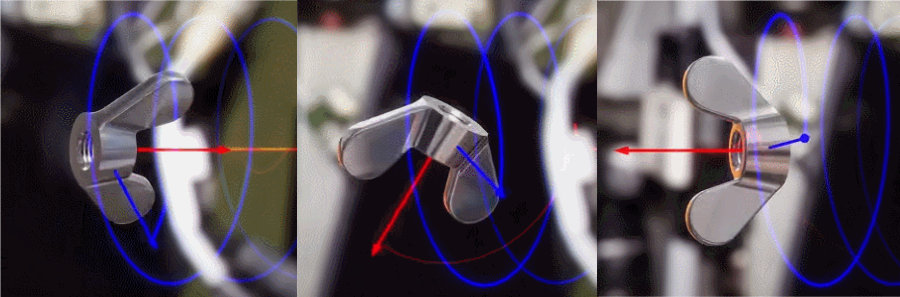
\includegraphics[width=0.9\textwidth]{dzhani.jpg}
\end{center}
   \caption{ジャニベコフ効果の描写 \cite{28}.}
\label{fig:10}
\end{figure*}

\begin{figure*}[b]
\begin{center}
% \fbox{\rule{0pt}{2in} \rule{.9\linewidth}{0pt}}
\includegraphics[width=1\textwidth]{layers.jpg}
\end{center}

   \caption{ECDO反転を引き起こす地球内部プロセスの描写 \cite{129}.}
\label{fig:11}
\end{figure*}

世界の主要な砂漠と生物多様性ホットスポットの位置もこのパターンと一致している。砂漠は堆積物で大きく覆われると予測される場所に存在し、生物多様性ホットスポットは海洋の変位の影響がそれほど大きくない場所に存在する\cite{28}。この配置は図\ref{fig:9}に示されている。

予測されるECDO回転経路へのこのような整列は、アメリカ西部の砂岩層に保存された堆積古流や、氷河によって運ばれたとされる漂礫岩(異なる岩石タイプの基盤岩上に移動・堆積した岩石)にも見られる\cite{21}。イギリスでは、これらの漂礫岩はECDO回転と一致する予想される流路に従っている\cite{67,68}。

\section{ECDO反転の原因となる物理学}

地球の自転軸が急激に変化する原理は、回転する物体の物理学にあります。その典型的な例がジャニベコフ効果であり、これはロシアの宇宙飛行士ウラジーミル・ジャニベコフによって発見され、図\ref{fig:10}に示されています。物体がその三つの主慣性軸のいずれかで完全に回転していない場合、固定された回転軸を維持できません。もし二番目の主慣性軸付近で回転していると、突発的な回転方向の変化が起こるように見えます。これは地球の急激な反転時に起こる現象そのものではありませんが、外力がなければ回転物理学のみが地球の自転軸の急激な変化を説明できるということが重要です。

正確に言えば、地球が単純で一様なジャニベコフ効果を経験することはほぼありません。もしそうであれば、地球の自転軸が時間をかけて徐々に変化するのを検出できるはずです。むしろ、地球は周期的で突発的な物理構造の乱れを経験し、「外側回転体」(地殻・マントル)と「内側回転体」(核)が分離(デカップリング)されると考えられています。外部からの入力がない場合、角運動量保存則により、地球は自転軸を急激に変化させることができません。したがって、外側回転体と内側回転体の分離は、外部からの衝撃を除いて、急激で突発的な反転を引き起こす数少ないプロセスのひとつとなります。

地球内部の乱れを引き起こす具体的なプロセスは、地球の核を構成する鉄の構造の状態変化であると考えられています(図\ref{fig:11})。内核は六方最密充填構造(hcp)の鉄(Fe)でできています\cite{141}。このhcp-Feが液体金属状態に変化すると、運動エネルギーを解放し、外核へと押し出されます。この相転移により核の磁気透過率が低下し、地磁気が弱くなり、熱が放出され、マントル内にLLVP(大規模低速度せん断領域)構造(図\ref{fig:12})\cite{38}が形成され、深海を介して地表を加熱します。これらの傾向は近年においてもよく記録されており、本論文の後半で詳しく論じます。

% \begin{figure*}[t]
% \begin{center}
% % \fbox{\rule{0pt}{2in} \rule{.9\linewidth}{0pt}}
% \includegraphics[width=0.45\textwidth]{llvp.jpg}
% \end{center}
%    \caption{南アフリカ下のLLVPの詳細なビジュアル \cite{28}.}
% \label{fig:18}
% \end{figure*}

\begin{figure}[t]
\begin{center}
% \fbox{\rule{0pt}{2in} \rule{0.9\linewidth}{0pt}}
   \includegraphics[width=1\linewidth]{llvp.jpg}
\end{center}
   \caption{南アフリカ下のLLVPの詳細なビジュアル \cite{28}.}
\label{fig:12}
\label{fig:onecol}
\end{figure}


地球内部でも同様のプロセスが逆方向で起こっていると考えられており、これによって反転後比較的早く地球の現在の自転状態への復帰が促進されると信じられている。

% \begin{figure}[t]
% \begin{center}
% % \fbox{\rule{0pt}{2in} \rule{0.9\linewidth}{0pt}}
%    \includegraphics[width=1\linewidth]{hcp.jpg}
% \end{center}
%    \caption{HCP-Fe から FCC-Fe への相転移により運動エネルギーが放出される \cite{28}.}
% \label{fig:11}
% \label{fig:onecol}
% \end{figure}

% \begin{figure}[t]
% \begin{center}
% % \fbox{\rule{0pt}{2in} \rule{0.9\linewidth}{0pt}}
%    \includegraphics[width=1\linewidth]{llvp-simple.jpg}

% \end{center}
%    \caption{地球のマントルにおけるLLVP(大規模低速度せん断領域)構造とその形成過程 \cite{28,39}.}
% \label{fig:12}
% \label{fig:onecol}
% \end{figure}

\section{地球反転が差し迫っている証拠}

私たちが再び地球反転の瀬戸際にいると信じる強い理由があります。何千年もの間、大災害は発生しておらず、これは歴史的記録やデータに基づいてこの種の出来事が起こる頻度とほぼ一致しています。差し迫る反転を支持する最も強力なデータは、最近の地磁気データであり、地球の地磁気が約二千年前から弱まり続けていることを示しています。この弱体化は加速しており、ここ数十年で深刻な水準に達しています。

図\ref{fig:14}には、1590年と2025年の地球の地磁気が示されています\cite{125,126}。図に示されているように、地磁気は著しく弱まっています。

地磁気の弱体化を示すもう一つの指標が地磁気北極の位置です(図\ref{fig:13})。地磁気北極は歴史的にカナダ北極圏に位置していました。しかし、過去数世紀の間、ゆっくりと移動しており、数十年前に大きく加速しました。現在は毎年55キロメートルの速さで急速にロシア方向へ移動しています\cite{124}。

\begin{figure}[b]
\begin{center}
% \fbox{\rule{0pt}{2in} \rule{1\linewidth}{0pt}}
   \includegraphics[width=1\linewidth]{npw.jpg}
\end{center}
   \caption{地磁気北極の位置(1590年から2025年まで)を5年ごとに示したもの \cite{142}.}
\label{fig:13}
\label{fig:onecol}
\end{figure}

\begin{figure*}[t]
\begin{center}
% \fbox{\rule{0pt}{2in} \rule{.9\linewidth}{0pt}}
\includegraphics[width=0.9\textwidth]{saa.jpg}
\end{center}
   \caption{1590年から2025年にかけての地磁気減少の様子。gufm1およびIGRF-14モデルを用いて計算\cite{125,126}.}
\label{fig:14}
\end{figure*}

\begin{figure}[t]
\begin{center}
% \fbox{\rule{0pt}{2in} \rule{1\linewidth}{0pt}}
   \includegraphics[width=1\linewidth]{ocean-highlight.jpg}
\end{center}
   \caption{深海($>$2000\,m)における1991年から2010年までの海洋昇温率。赤で囲まれている \cite{132}.}
\label{fig:15}
\label{fig:onecol}
\end{figure}

地球の磁場は、地球の回転によって外核内で動くマグマの流れの円柱(内なるダイナモ)によって生成されていると考えられている\cite{123}。地磁気の弱体化は、地球内部深部での撹乱の症状である。ECDO理論によれば、これらの撹乱によって熱が排出され、最終的にはマントルと核の切り離しを引き起こし、地球反転が発生する\cite{1}。

内なる地球で発生する発熱反応プロセスの存在を裏付ける多くのデータが存在する。地球の温暖化は、大陸および海洋の表層温度の上昇\cite{127,128}、地球内部からの熱流と同期して変動する大気中CO2濃度の上昇\cite{129,130}、そして全球海氷面積の減少\cite{131}として記録されている。これらのデータは、CO2濃度や気温の上昇が「人為的」気候変動の原因ではなく、むしろ発熱性コアの下流効果であることを示唆している\cite{129}。

特に重要なのは、深海(深さ$>$2000メートル)の温暖化率の研究である。深海が温暖化しているだけでなく、最も強い温暖化がアビサル層(4000〜6000m)で観測されている。この深海温暖化の中心は4000メートル以下に位置しており\cite{132,129}、もし大気によって上から加熱されているのであれば説明がつかない。これらのデータは、近年の気候変動や地磁気変動が地球深部のプロセスによって駆動されていることを強く支持している。図\ref{fig:15}は、1991年から2010年の全球深海温暖化率を示す\cite{132}。

\section{差し迫る地球反転のモデリング}

地球の次の反転のタイミングを予測することは複雑な課題です。現在、この現象に関する最良のモデルは地球の地磁気場、特に南大西洋異常帯(SAA)にあります。この南大西洋上の領域は最も地磁気場が弱く、32,000ナノテスラ未満の場の強さの領域として定義されています\cite{135}。これは1590年における最弱の場の値でした。南大西洋異常帯の面積は、1590年の地球表面の1\%から2025年には21\%に増加しています\cite{136}。

地球がいつ反転するかを推定するために、私はSAA面積のデータをべき乗則のティッピングポイント方程式に当てはめました。これは、複雑なシステムが臨界値に近づくにつれ、劇的かつ急激な変化が発生することをモデル化するものです。私の計算によると、予測される臨界転換日は2059年3月13日となりました(図\ref{fig:16})。この予測は、転換点に近づくにつれてより正確になるでしょう\cite{136}。

自転軸の変動、気象異常、地震や火山活動などの他の指標も、次の地球反転がいつ起こるかの予測精度を高めるのに役立ちます。

\begin{figure}[t]
\begin{center}
% \fbox{\rule{0pt}{2in} \rule{1\linewidth}{0pt}}
   \includegraphics[width=1\linewidth]{saa-crop.jpeg}
\end{center}
   \caption{南大西洋異常点に基づくティッピングポイントの計算によれば、2059年3月13日が示唆されている\cite{125,126}。}
\label{fig:16}
\label{fig:onecol}
\end{figure}

\section{ECDO 歴史年表}

過去のECDOイベントについて正確な年表を確立することは困難ですが、完新世には少なくとも2回のECDOイベントがあったようです。ヘロドトスがエジプトの神官から聞いた話に注目してください。すなわち、\textit{「最初の王から最後のヘパイストスの神官まで341代の人々がいた…この間に太陽は4回、その昇る位置を変え、今沈んでいる場所から2回昇り、今昇る場所から2回沈んだと言われている」}\cite{32}。紀元前5世紀に生きたプラトン\cite{111}は、アトランティスが一昼夜で沈んだ大洪水(約9000年前)の後、\textit{「それ以来、多くの洪水があり、山中で生き残った者たちは書く術を知らず、長い世代にわたり生きる手段を手に入れることに専念していた」}\cite{112}と述べています。これは、約9700年前のヤンガードリアス期以降に2回以上の反転があったことを示唆しています。本論文および私の研究\cite{2}で示される物理的証拠は、プラトンの記述を裏付けています。

最近のECDO反転の候補日は紀元前2300年から紀元前1600年の間であり、多くの大洪水伝承(禹の治水\cite{113,114,115}、オギュゲス\cite{116,117}、ペルー\cite{118,119}、出エジプト記\cite{120})、文明の崩壊や放棄(モヘンジョダロ\cite{121}、ミノア・クレタ\cite{100,101})、そして物理的異常(ボンドイベント\cite{122}、4.2キロ年イベント\cite{90})がこの時期に帰属されています。これ以降に大規模な破局的出来事があったことを示す十分な証拠の収束はありません。

\section{結論}

ナヌーク作戦は、第二次世界大戦後にアメリカ合衆国が北極およびソ連北部沿岸の地図作成のために実施した冷戦期の偵察事業でした\cite{137}。調査の過程で、磁極が従来の調査結果よりも125〜200マイル北にあることが発見されました。これを受けて、\textit{「政府の科学者たちの間で、磁極と地理極が一致したとき何が起こるかという疑問が生じた。これに答えるため、ポール・A・サイプル博士のプロジェクト管理のもと、ランド社に依頼して、同心球モデルによる地球の実験室研究が行われた。内球は電磁的に帯電した溶融鉄の核、軸が“磁極”を定義し、外球は地殻で、“地理極”軸を中心に回転する仕組みであった。繰り返しの実験から、“磁極”が“地理極”に近づくと、遠心力に引かれたかのように収束速度が加速し一致しそうになるが、実際には一致するのではなく、“磁極”が“地理極”の周囲を急速に“反転(フリップ)”し、その後遠心力で赤道方面へ跳ね飛び、二つの軸の差が約89度となる場所に移動することが判明した。この極の“反転”が起きた後、軸は長い時間をかけて再び徐々に収束し始める」}\cite{138,139}。

その後、\textit{「1948年初頭、ホワイト少佐が出席したペンタゴンでの科学者会議のひとつで、科学者たちはこの極反転現象について一般市民に警告すべきかを議論した。誰もこの情報を秘匿にすることには同意しなかったが、どう発表するかにも合意できなかった。この現象の知識は、社会の道徳的基盤を破壊する可能性があると感じていた者もいた。しかし、その懸念は1950年代初頭に新聞コラムや雑誌記事でこの反転現象情報が公開された際、驚くほど無反応、あるいは茫然自失・不信感に満ちた市民から何の反応も生じなかったことで、根拠のないものだったことがわかった」}\cite{138,139}。

なぜ私たちはこのことについて注意を払わないのでしょうか?地球がこれまでに反転したと考える十分な理由があります。本論文と続編は、世界中の洪水伝承、大陸を覆う岩塩や海洋化石、古代の地下避難施設、動物遺骸、破局的地形など、多方面から集まる多数の証拠の濃密な要約を提供しています。人類は数十万年前から存在するとされるのに、現代史はほんの数千年前に遡るにすぎません。もしかすると、定期的に地球が反転し、大陸が一掃され、私たちが再びゼロ(石器時代)に戻り、古代史の記録が数少ない破局的伝承だけになる、ということがあったのではないでしょうか?もしそうだとすれば、これを再び防ぐことは人類の最重要課題の一つなのかもしれません。
最後に、イシャルは、プラトンが著した『ティマイオス』に記された、アテネの政治家ソロンとエジプトの僧侶たちとの会話のエピソードを、ここに紹介する \cite{140}: \textit{「最後に、プラトンによって書かれた『ティマイオス』に記された、アテナイの政治家ソロンとエジプトの神官たちとの間で交わされた会話を紹介します。ある時、ソロンが彼らに古代史について話すように仕向けようとして、フォロネウスが最初の人間であったという私たちの最も古い伝承や、ニオベについての話、そして大洪水の後にデウカリオーンとピュラがどのように生き残ったかについての伝説、さらにその子孫の系譜について語り、これらの出来事に要した年数から時代を計算しようとしました。すると、その神官の一人で年老いた男がこう言いました。「ソロンよ、ソロンよ、ギリシャ人はいつも子供のようである。年老いたギリシャ人など存在しないのだ」と。これを聞いたソロンが「どういう意味か」と問いただすと、神官は「お前たちは魂が若いのだ。一人残らず。お前たちの中には、古くから伝わる信仰もなければ、時を経た学問もない。それには理由がある。過去にもこれからも、人類には様々な滅亡があり、それらの中でも最大のものは火と水によるものであり、他にも無数の手段によるものがある。実は、お前の国や我々の国でも語り継がれているファエトンの伝説――太陽神ヘリオスの子が父の戦車を駆り、操ることができず地上の全てを焼き尽くし、雷に撃たれて滅んだという話――も、伝説の形をとってはいるが、実際は天体の軌道の変動による地上の火災と、それが長い周期で繰り返される事実に基づいているのだ。そのような時には、高地や乾燥した土地に住む者たちが河川や海の近くに住む者よりも大きな被害を受ける。我々の場合、ナイル川は普段は様々な恵みをもたらすが、そのような時にもこの災厄から我々を救ってくれる。そして神々が大洪水で大地を清める時には、山中の牧人や羊飼いは助かるが、お前たちの国の都市にいる者たちは川の流れに押し流されて海に沈む。しかし我々の国では、その時も他の時も、水が大地を上から押し流すことはなく、むしろ下から自然に湧き出してくるのだ。だから、ここに保存されているものが最も古いとされている。本当は、極端な暑さや寒さがなければ、どこでも必ず人類の系譜が存在し、数が多かったり少なかったりするのだ。そして、もしもどこかで偉大な出来事、善なる出来事、目立つ出来事が起きた場合、それが我々の国であれ、お前たちの国であれ、あるいは他の伝え聞く場所であれ、すべてそのような出来事は神殿で古くから記録され、保存されている。一方、お前たちや他の人々は、そのたびごとに文字やあらゆる技芸を一から手に入れ、普通の年月が経過した後には、まるで疫病のように天からの洪水が再び襲い、教養も学問も持たぬ者以外を残らず失ってしまうのだ。だから再び一からやり直し、昔この国や自国で起きた出来事を何も知らぬまま若くなってしまう。確かに今話したお前たちの系譜――ソロンよ、お前の国の系譜――は子供の話より少しはましという程度だ。なぜなら、そもそも一度の大洪水しか覚えていないが、実際は以前にも多く起こっているのだ。さらに最も高貴で完全無欠な人々が、お前たちが今住む土地で生まれ、お前もお前たちの都市も、そこから生き残ったほんのわずかな種から生まれたことも知らない。だが多くの世代にわたり、生き残った者たちは書き記す術を持たなかったため、そのことを忘れてしまったのだ。かつて大洪水による最大の滅亡よりも前には、今のアテナイ国家は戦争において最も勇敢であり、また他のあらゆる点でもきわめて秩序立っていたと言われている。最も美しい芸術と、高貴な政治制度を持つ国であったと伝えられている。」}

これらの祭司たちは、当然ながらソロンにアトランティスの古代文明についても語った: \textit{「もちろん、これらの神官たちは、ソロンにアトランティスの古代文明についても語った。「ここの入り江の中にあるものは、明らかに狭い入口を持つ港にすぎない。しかしあちらに広がるのは本当の大海原であり、それを囲む大地こそ、真に大陸と呼ぶにふさわしい。さて、このアトランティス島には、強大かつ驚くべき力を持った王たちの同盟が存在し、島全体はもとより、他の多くの島々や大陸の一部にまで支配力を及ぼしていた。そして、ここヘラクレスの柱内側の土地でも、リビアはエジプトに至るまで、ヨーロッパはテュルレニアに至るまでその支配を広げていた。この大軍が一度だけ、あなたの国と我々の国、そしてヘラクレスの柱内側のすべての地を一度に征服しようと企てたのだ。その時こそ、ソロンよ、あなたがたアテナイの人々が世界の前で勇気と力を最も鮮やかに示した。全てにおいて勇敢さと戦いの技が際立ち、ギリシャの指導者として、あるいは他の全ての者に見捨てられても独りで立ち向かい、死の危険を乗り越えて侵略者を打ち破り、記念のトロフィーを建てた。まだ奴隷になっていなかった者たちを奴隷化から救い、我々ヘラクレスの柱内に住む全ての人々を惜しみなく解放してくれたのだ。しかしその後、不吉な地震や洪水が起こり、悲惨な一昼夜が訪れ、あなた方の戦士たちは一人残らず大地に呑まれ、アトランティス島もまた同様に海に沈み、消え失せたのである。」}

\section{謝辞}

The Ethical Skeptic(ECDO論文のオリジナル著者)には洞察に富み、画期的な論文を完成させ、世界と共有してくださったことに感謝します。彼の三部作論文 \cite{1} は、エクソサーミック・コア・マントル・デカップリング・ジャニベコフ・オシレーション(ECDO)理論の基礎となる重要な著作であり、私がここで簡潔に述べた内容よりも、このテーマに関するはるかに多くの情報を包含しています。

Ankit氏に感謝します。彼は表1のcataclysm com-pilationデータを処理してくれました。

そしてもちろん、私たちが肩に乗っている偉大な皆様に感謝します。この研究を可能にしたすべての研究と調査を行い、人類に光を照らすために尽力された方々です。

\clearpage
\twocolumn

\section{その他画像}

% \begin{figure*}[b]
% \begin{center}
% % \fbox{\rule{0pt}{2in} \rule{.9\linewidth}{0pt}}
% \includegraphics[width=1\textwidth]{layers.jpg}
% \end{center}
%    \caption{ECDOの反転を引き起こす地球内部プロセスの描写 \cite{129}.}
% \label{fig:17}
% \end{figure*}

% \begin{figure*}[b]
% \begin{center}
% % \fbox{\rule{0pt}{2in} \rule{.9\linewidth}{0pt}}
% \includegraphics[width=0.45\textwidth]{llvp.jpg}
% \end{center}
%    \caption{南アフリカ下のLLVPの詳細な可視化 \cite{28}.}
% \label{fig:18}
% \end{figure*}

% \begin{figure}[t]
% \begin{center}
% % \fbox{\rule{0pt}{2in} \rule{1\linewidth}{0pt}}
%    \includegraphics[width=1\linewidth]{llvp.jpg}

\begin{figure}[H]
\begin{center}
% \fbox{\rule{0pt}{2in} \rule{1\linewidth}{0pt}}
   \includegraphics[width=1\linewidth]{wave.jpg}
\end{center}
   \caption{カフラー王のピラミッドに見られる、波状の侵食(アンダーカット、放物線状の波による侵食)を詳しく観察した様子 \cite{27}。}
\label{fig:19}
\label{fig:onecol}
\end{figure}

\begin{figure}[H]
\begin{center}
% \fbox{\rule{0pt}{2in} \rule{1\linewidth}{0pt}}

   \includegraphics[width=1\linewidth]{star-stone.jpg}
\end{center}
   \caption{クフ王のピラミッドのシャフトの一つに彫られた星図 \cite{28}.}
\label{fig:20}
\label{fig:onecol}
\end{figure}

% \begin{figure}[t]
% \begin{center}
% % \fbox{\rule{0pt}{2in} \rule{1\linewidth}{0pt}}
%    \includegraphics[width=1\linewidth]{deepsea.jpg}
% \end{center}
%    \caption{深海}
% \label{fig:16}
% \label{fig:onecol}
% \end{figure}

\begin{figure*}[t]
\begin{center}
% \fbox{\rule{0pt}{2in} \rule{.9\linewidth}{0pt}}

\includegraphics[width=1\textwidth]{deepsea.jpg}
\end{center}
   \caption{深海および超深海の加熱異常と通常の大気海洋加熱曲線を比較したビジュアルです。全体的な加熱異常はNOAAより取得\cite{147}、深海および超深海の加熱分布はDesbruyeresの研究\cite{132}、データ処理と可視化は倫理的懐疑論者(The Ethical Skeptic)によるものです\cite{129}。}
\label{fig:21}
\end{figure*}

\begin{figure*}[t]
\begin{center}
% \fbox{\rule{0pt}{2in} \rule{.9\linewidth}{0pt}}
\includegraphics[width=1\textwidth]{sealevel.jpeg}
\end{center}
   \caption{海面は63観測所において75年間で分散が20\%増加しており、海流速度の上昇を示しています。海面分散の急上昇は海洋の熱パルスと同時に発生しており、これらは地球深部の加熱によって引き起こされている可能性があります\cite{2,129}。}
\label{fig:22}
\end{figure*}

\begin{figure*}[t]
\begin{center}
% \fbox{\rule{0pt}{2in} \rule{.9\linewidth}{0pt}}
\includegraphics[width=1\textwidth]{co2.jpg}
\end{center}
   \caption{大気中のCO2濃度(ppm)は過去45年間一貫して上昇しており、その原因は海洋温度の上昇と考えられます。出典:NOAA \cite{148,129}.}
\label{fig:23}
\end{figure*}

\begin{figure*}[t]
\begin{center}
% \fbox{\rule{0pt}{2in} \rule{.9\linewidth}{0pt}}
\includegraphics[width=1\textwidth]{ice.jpg}
\end{center}
   \caption{地球規模の海氷面積は過去45年間で縮小しており、これは地球温暖化によるものです。出典:ADS \cite{149}.}
\label{fig:24}
\end{figure*}

% \begin{figure}[t]
% \begin{center}
% % \fbox{\rule{0pt}{2in} \rule{1\linewidth}{0pt}}
%    \includegraphics[width=1\linewidth]{co2.jpg}
% \end{center}
%    \caption{co2}
% \label{fig:16}

% \label{fig:onecol}
% \end{figure}

% \begin{figure}[t]
% \begin{center}
% % \fbox{\rule{0pt}{2in} \rule{1\linewidth}{0pt}}
%    \includegraphics[width=1\linewidth]{ice.jpg}
% \end{center}
%    \caption{氷}
% \label{fig:16}
% \label{fig:onecol}
% \end{figure}

%-------------------------------------------------------------------------
%-------------------------------------------------------------------------
%-------------------------------------------------------------------------
%-------------------------------------------------------------------------
%-------------------------------------------------------------------------
%-------------------------------------------------------------------------
%-------------------------------------------------------------------------
%-------------------------------------------------------------------------
%-------------------------------------------------------------------------
%-------------------------------------------------------------------------
%-------------------------------------------------------------------------
%-------------------------------------------------------------------------
%-------------------------------------------------------------------------
%-------------------------------------------------------------------------
%-------------------------------------------------------------------------
%-------------------------------------------------------------------------
\clearpage
\twocolumn

{\small
\renewcommand{\refname}{参考文献}
\bibliographystyle{ieee}
\bibliography{egbib}
}

\end{document}